\documentclass[12pt]{article}
\usepackage[
  top=2.50cm,
  bottom=1.50cm,
  left=1.50cm,
  right=1.50cm
]{geometry} 
\usepackage{amsmath,amsthm,amssymb}
\usepackage{algorithm,algorithmic}
\usepackage{graphicx}
\usepackage{tikz}

\newenvironment{theorem}[2][Theorem]{\begin{trivlist}
\item[\hskip \labelsep {\bfseries #1}\hskip \labelsep {\bfseries #2.}]}{\end{trivlist}}
\newenvironment{lemma}[2][Lemma]{\begin{trivlist}
\item[\hskip \labelsep {\bfseries #1}\hskip \labelsep {\bfseries #2.}]}{\end{trivlist}}
\newenvironment{exercise}[2][Exercise]{\begin{trivlist}
\item[\hskip \labelsep {\bfseries #1}\hskip \labelsep {\bfseries #2.}]}{\end{trivlist}}
\newenvironment{problem}[2][Problem]{\begin{trivlist}
\item[\hskip \labelsep {\bfseries #1}\hskip \labelsep {\bfseries #2.}]}{\end{trivlist}}
\newenvironment{question}[2][Question]{\begin{trivlist}
\item[\hskip \labelsep {\bfseries #1}\hskip \labelsep {\bfseries #2.}]}{\end{trivlist}}
\newenvironment{corollary}[2][Corollary]{\begin{trivlist}
\item[\hskip \labelsep {\bfseries #1}\hskip \labelsep {\bfseries #2.}]}{\end{trivlist}}

\begin{document}

\title{Homework 6}
\author{Thomas Kim~tsk389~51835\\David Munoz~dam2989~51840\\
CS331 Algorithms and Complexity}

\renewcommand{\arraystretch}{2.0}

\date{} % Suppress the datn{minipage}{0.5\textwidth}

% ------------------
% Begin Cover Page
% ------------------

\maketitle
% ------------------
% Begin Homework
% ------------------

\onecolumn

\begin{problem}
    {Q1: 13.2}
    Consider a county in which 100,000 people vote in an election.
    There are only two candidates on the ballot: a Democratic candidate (denoted $D$) and
    and Republican candidate $R$. As it happens, this county is heavily Democratic, so 80,000
    people go to the polls with the intention of voting for $D$, and 20,000 go to the polls with the intention of voting for $R$.\\

    However, the layout of the ballot is a little confusing, so each voter, independently and with probability $\frac{1}{100}$, votes for the
    wrong candidate - that is, the one that he or she \textit{didn't} intend to vote for.
    (Remember that in this election, there are only two candidates on the ballot.)\\

    Let $X$ denote the random variable equal to the number of votes received by the Democratic candidate $D$ when the voting is conducted with this
    process of error. Determine the expected value of $X$, and give an explanation of your derivation of this value.
\end{problem}

\begin{problem}
    {Q2}
    Is the set of rational numbers countably infinite or uncountably infinite? \\
    \textbf{Countably Infinite} \\
    \begin{proof}
        Let $r \in \mathbb{Q}$ be a rational number. \\
        Consider rational numbers of the form $\frac{a}{b}$ where $a \in \mathbb{Z} \land b \in \mathbb{Z}_{\geq 0} \land gcd(a,b) = 1$ \\
        Claim: All rational numbers $\frac{q}{r}, q, r \in \mathbb{Z}$ can be expressed in this form. \\
        First, factor out $-1$ from all negative $q, r$, such that the number is expressed $s\frac{|q|}{|r|}$ where $s = (-1)^1 \lor s = (-1)^2$ \\
        Next, divide $q, r$ by $gcd(q, r)$ such that the number is expressed $s \frac{|q'|}{|r'|}$ where $q', r'$ are the result after dividing $q, r$ by $gcd(q, r)$ \\
        By the definition of gcd, $q', r'$ share no common prime factors \\
        Now, define a mapping $f: \mathbb{Q} \rightarrow \mathbb{Z} \times \mathbb{N}$ as follows: \\
        $f(\frac{a, b}) = (a, b)$ \\
        This mapping is clearly onto, as every Cartesian pair can be mapped to a corresponding real number by taking $(a,b) \rightarrow \frac{a}{b}$ \\
        The cartesian product of $\mathbb{Z} \times \mathbb{N}$ is countably infinite \\
        Therefore, the rational numbers are countably infinite. \\
    \end{proof}
\end{problem}

\begin{problem}
  {Q3(a)}
  ~\\
  \begin{center}
    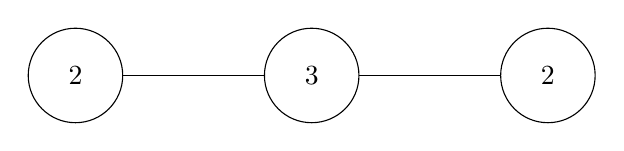
\begin{tikzpicture}[scale=0.2]
      \tikzstyle{every node}+=[inner sep=0pt]
      \draw [black] (5,0) circle (3);
      \draw (5,0) node {$2$};
      \draw [black] (20,0) circle (3);
      \draw (20,0) node {$3$};
      \draw [black] (35,0) circle (3);
      \draw [black] (35,0) node {$2$};
      \draw [black] (23,0) -- (32,0);
      \draw [black] (8,0) -- (17,0);
    \end{tikzpicture}
  \end{center}
  In this example, the middle node will be chosen and the two side nodes discarded for a total weight of $3$. \\
  If the middle node was discarded and the two side nodes chosen, the total weight would have been $4 > 3$. \\
\end{problem}

\begin{problem}
  {Q3(b)}
  ~\\
  \begin{center}
    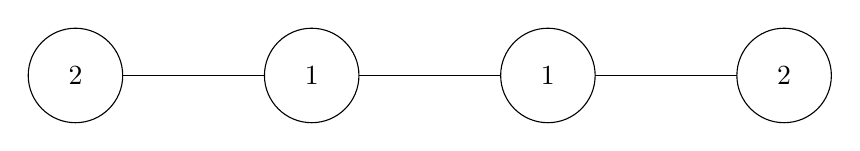
\begin{tikzpicture}[scale=0.2]
      \tikzstyle{every node}+=[inner sep=0pt]
      \draw [black] (5,0) circle (3);
      \draw (5,0) node {$2$};
      \draw [black] (20,0) circle (3);
      \draw (20,0) node {$1$};
      \draw [black] (35,0) circle (3);
      \draw (35,0) node {$1$};
      \draw [black] (50,0) circle (3);
      \draw (50,0) node {$2$};
      \draw [black] (8,0) -- (17,0);
      \draw [black] (23,0) -- (32,0);
      \draw [black] (38,0) -- (47,0);
    \end{tikzpicture}
  \end{center}
  In this example, the maximum weight independent set includes nodes $v_1$ and $v_4$, but $1$ is odd and $4$ is even. \\
\end{problem}

\begin{problem}
    {Q4(a)}
    Given $n$ containers of weight $w_1, \dots, w_n$, trucks of capacity $K$, minimize the number of trucks to carry all the weight. This problem is NP-Complete. \\
    Greedy Algorithm: Start with an empty truck, then begin piling containers $1, 2, 3, \dots$ until you get to a container which would overflow the weight limit. \\
    Now declare this truck "loaded" and send it off; then continue the process with a fresh truck. \\
    Given an example of a set of weights, a value of $K$, where this algorithm does not use the minimum possible number of trucks. \\
    \begin{proof}
        Let $K = 3$, $w_1, \dots, w_{\frac{n}{2}} = 2, w_{\frac{n+2}{2}}, \dots, w_n = 1$, $n \geq 4$, $n$ is even \\
        Trivially, the ideal arrangement would be to have each truck carry one container of weight $2$ and one of weight $1$ to fully utilize every truck. \\
        However, the first truck will be loaded with weight $w_1 = 2$, then $w_2 = 2$ would overload it, so it will leave with only weight 2. \\
    \end{proof}
\end{problem}

\begin{problem}
    {Q4(b)}
    Show, however, that the number of trucks used by this algorithm is within a factor of $2$ of the minimum possible number, for any set of weights and any value $K$ \\
    \begin{proof}
        Claim: The average utilization of each truck will not be below $\frac{1}{2}$ \\
        Suppose some truck currently carrying weight $a$ cannot accept $w_i$, because $w_i + a > K$ \\
        This means $a > K - w_i$ by definition. \\
        The minimum usage of this truck would therefore be $\frac{K - w_i + 1}{K}$ \\
        The next truck is guaranteed to use at least $b = w_i$ weight, since it is initially empty and $w_i$ is the first container to be loaded. \\
        Therefore, the average utilization of these two trucks is $\frac{1}{2}\left(\frac{K - w_i + 1}{K} + \frac{w_i}{K}\right)$ \\
        $= \frac{K + 1}{2K} > \frac{K}{2K} = \frac{1}{2}$ \\
        Extending this, the average usage of any arbitrary adjacent pair of trucks is guaranteed to be at least $\frac{1}{2}$ \\
        Now, given a container assignment, choose adjacent pairs such that each pair is disjoint from all other pairs. \\
        Given $N$ trucks used, this situation is equivalent to having $N$ trucks each using precisely $\frac{1}{2}$ of their max capacity. \\
        The lower bound for the minimum number of trucks $N_m$ trivially occurs when all trucks use precisely $100\%$ of their max capacity. \\
        So given that each truck, in the worst situation with the greedy algorithm, use at least $50\%$ of their max capacity, the number of trucks
        used by the greedy algorithm must be within a factor of $2$ of the minimum possible number. \\
    \end{proof}
\end{problem}

\begin{problem}
  {Q5}
  Consider a set of mobile computing clients in a certain town who each need to be connected to one of several possible \textit{base stations}.
  We'll suppose there are $n$ clients, with the position of each client specified by its $(x,y)$ coordinates in the plane. There are also $k$ base stations; the positions
  of each of these is specified by $(x,y)$ coordinates as well. For each client, we wish to connect it to exactly one of the base stations. Our
  choice of connections is constrained in the following ways.\\
  \begin{itemize}
  \item There is a \textit{range parameter} $r$ - a client can only be connected to a base station that is within distance $r$.
  \item There is also a \textit{load parameter} $L$ - no more than $L$ clients can be connected to any single base station.
  \end{itemize}
  Your goal is to design a polynomial-time algorithm for the following problem. Given the positions of a set of clients and a set of base stations, as well as the range and load parameters, decide
  whether every client can be connected simultaneously to a base station, subject to the range and load conditions in the previous paragraph.
  \begin{algorithmic}[1]
    \STATE Create a graph $G(V, E)$
    \STATE Let some edge $e(a, b)_w$ be a directed edge from $a$ to $b$ with weight $w$
    \STATE Let the set of clients be denoted $C = \{c_1, c_2, \dots, c_n\}$
    \STATE Let the set of base stations be denoted $B = \{b_1, b_2, \dots, b_n\}$
    \STATE Define the function $valid(c_i)$ to return some set $B' = \{b'_1, b'_2, \dots, b'_n\} \subset B$ such that $c_i$ is within range $\forall b_i \in B'$
    \STATE $V = \{s, t, c_1, c_2, \dots, c_n, b_1, b_2, \dots, b_n\}$
    \STATE Initially $E = \{\}$
    \FOR {$\forall v_i \in V$}
    \IF {$v_i \in C$}
    \STATE $B' = valid(v_i)$
    \STATE $E = E \cup \{(s, v_i)_1, (v_i, b'_1)_1, \dots, (v_i, b'_n)_1\}$
    \ENDIF
    \IF {$v_i \in B$}
    \STATE $E = E \cup \{(b_i, t)_{L_{b_i}}\}$
    \ENDIF
    \ENDFOR
    \STATE Run Ford-Fulkerson on $G$ to find maximum flow $f$
    \IF {$f = n$}
    \RETURN TRUE
    \ELSE
    \RETURN FALSE
    \ENDIF
  \end{algorithmic}
  \noindent
  \textbf{Correctness}
  \begin{proof}
  \end{proof}
  \noindent
  \textbf{Runtime}
  \begin{proof}
  \end{proof}
\end{problem}


% -----------------
% End Homework
% -----------------

\end{document}
